% Created 2023-09-14 Thu 11:34
% Intended LaTeX compiler: xelatex
\documentclass[xcolor=table,10pt,aspectratio=169]{beamer}

\RequirePackage{etex}
\RequirePackage[l2tabu,orthodox]{nag}            %% Warn about obsolete commands and packages
\RequirePackage{amsmath,amsfonts,amssymb,amsthm} %% Math
\RequirePackage{ifxetex,ifluatex}                %% Detect XeTeX and LuaTeX
\RequirePackage{fixltx2e}                        %% provides \textsubscript
\RequirePackage{xspace}
\RequirePackage{graphicx}
\RequirePackage{comment}
\RequirePackage{url}
\RequirePackage{relsize}
\RequirePackage{booktabs}
\RequirePackage{tabularx}
\RequirePackage[normalem]{ulem}
\RequirePackage[all]{xy}
\RequirePackage{etoolbox}

%%%
%%% Code Listings
%%%

\RequirePackage{listings}
\lstdefinelanguage{Sage}[]{Python}{morekeywords={True,False,sage,cdef,cpdef,ctypedef,self},sensitive=true}

\lstset{frame=none,
  showtabs=False,
  showspaces=False,
  showstringspaces=False,
  commentstyle={\color{gray}},
  keywordstyle={\color{mLightBrown}\textbf},
  stringstyle ={\color{mDarkBrown}},
  frame=single,
  basicstyle=\tt\scriptsize\relax,
  backgroundcolor=\color{gray!190!black},
  inputencoding=utf8,
  literate={…}{{\ldots}}1,
  belowskip=0.0em,
}

\makeatletter
\patchcmd{\@verbatim}
  {\verbatim@font}
  {\verbatim@font\scriptsize}
  {}{}
\makeatother


%%%
%%% Pseudocode
%%%

\let\nl\undefine
\let\procedure\relax
\let\endprocedure\relax
\usepackage{algorithm2e}

%%%
%%% Tikz
%%%

\RequirePackage{tikz,pgfplots}
\pgfplotsset{compat=newest}

\usetikzlibrary{calc}
\usetikzlibrary{arrows}
\usetikzlibrary{automata}
\usetikzlibrary{positioning}
\usetikzlibrary{decorations.pathmorphing}
\usetikzlibrary{backgrounds}
\usetikzlibrary{fit,}
\usetikzlibrary{shapes.symbols}
\usetikzlibrary{chains}
\usetikzlibrary{shapes.geometric}
\usetikzlibrary{shapes.arrows}
\usetikzlibrary{graphs}

%% Cache but disable by default

\usetikzlibrary{external}
\tikzset{external/export=false}

\definecolor{DarkPurple}{HTML}{332288}
\definecolor{DarkBlue}{HTML}{6699CC}
\definecolor{LightBlue}{HTML}{88CCEE}
\definecolor{DarkGreen}{HTML}{117733}
\definecolor{DarkRed}{HTML}{661100}
\definecolor{LightRed}{HTML}{CC6677}
\definecolor{LightPink}{HTML}{AA4466}
\definecolor{DarkPink}{HTML}{882255}
\definecolor{LightPurple}{HTML}{AA4499}
\definecolor{DarkBrown}{HTML}{604c38}
\definecolor{DarkTeal}{HTML}{23373b}
\definecolor{LightBrown}{HTML}{EB811B}
\definecolor{LightGreen}{HTML}{14B03D}
\definecolor{DarkOrange}{HTML}{FFDD00}

\pgfplotsset{width=1.0\textwidth,
  height=0.6\textwidth,
  cycle list={%
    solid,LightGreen,thick\\%
    dotted,LightRed,very thick\\%
    dashed,DarkBlue,thick\\%
    dashdotted,DarkPink,thick\\%
    dashdotdotted,LightGreen,thick\\%
    loosely dotted,very thick\\%
    loosely dashed,DarkBlue,very thick\\%
    loosely dashdotted,DarkPink,very thick\\%
    \\%
    DarkBrown,thick\\%
  },
  legend pos=north west,
  legend cell align={left}}

\pgfplotsset{select coords between index/.style 2 args={
    x filter/.code={
        \ifnum\coordindex<#1\def\pgfmathresult{}\fi
        \ifnum\coordindex>#2\def\pgfmathresult{}\fi
    }
}}

%%%
%%% SVG (Inkscape)
%%%

\ifxetex % chktex 1
\providecommand{\executeiffilenewer}[3]{%
  {\immediate\write18{#3}} % hack
}
\else
\providecommand{\executeiffilenewer}[3]{%
  \ifnum\pdfstrcmp{\pdffilemoddate{#1}}%
    {\pdffilemoddate{#2}}>0%
    {\immediate\write18{#3}}
  \fi%
}
\fi

\providecommand{\includesvg}[2][1.0\textwidth]{%
 \executeiffilenewer{#1.svg}{#1.pdf}%
 {inkscape -z -D --file=#2.svg --export-pdf=#2.pdf --export-latex --export-area-page}%
 \def\svgwidth{#1} 
 \input{#2.pdf_tex}%
} 

%%%
%%% Metropolis Theme
%%%

\usetheme{metropolis}
\metroset{color/block=fill}
\metroset{numbering=none}
\metroset{outer/progressbar=foot}
\metroset{titleformat=smallcaps}

\setbeamercolor{description item}{fg=mLightBrown}
% \setbeamerfont{alerted text}{series=\bfseries}
\setbeamerfont{footnote}{size=\scriptsize}
\setbeamercolor{example text}{fg=mDarkBrown}
\setbeamercolor{block title alerted}{fg=white, bg=mDarkBrown}
\setbeamertemplate{bibliography item}[text]
% https://tex.stackexchange.com/questions/683533/beamer-theme-metropolis-does-not-allow-different-font-size-for-fullcite
\setbeamerfont{bibliography entry title}{size=}
\setbeamerfont{bibliography entry author}{size=}
\setbeamerfont{bibliography entry location}{size=}
\setbeamerfont{bibliography entry note}{size=}


\renewcommand*{\UrlFont}{\ttfamily\relax}

%%%
%%% UTF-8 & Fonts
%%% 

\RequirePackage{unicodesymbols} % after metropolis which loads fontspec

\setmonofont[BoldFont={Cousine Bold},
             ItalicFont={Cousine Italic},
             BoldItalicFont={Cousine Bold Italic},
             Scale=0.9]{Cousine}             
%%%
%%% BibLaTeX
%%%

\RequirePackage[backend=bibtex,
            style=alphabetic,
            maxnames=8,maxbibnames=8,maxalphanames=8,
            citestyle=alphabetic]{biblatex}

\bibliography{local.bib,abbrev3.bib,crypto_crossref.bib,rfc.bib,jacm.bib,dcc.bib}

\DeclareFieldFormat{title}{\alert{#1}}
\DeclareFieldFormat[book]{title}{\alert{#1}}
\DeclareFieldFormat[thesis]{title}{\alert{#1}}
\DeclareFieldFormat[inproceedings]{title}{\alert{#1}}
\DeclareFieldFormat[incollection]{title}{\alert{#1}}
\DeclareFieldFormat[article]{title}{\alert{#1}}
\DeclareFieldFormat[misc]{title}{\alert{#1}}

%%% 
%%% Microtype
%%%

\IfFileExists{upquote.sty}{\RequirePackage{upquote}}{}
\IfFileExists{microtype.sty}{\RequirePackage{microtype}}{}

\setlength{\parindent}{0pt}                   %%
\setlength{\parskip}{6pt plus 2pt minus 1pt}  %%
\setlength{\emergencystretch}{3em}            %% prevent overfull lines
\setcounter{secnumdepth}{0}                   %%

%%%
%%% Maths
%%%

\DeclareMathOperator{\Vol}{Vol}
\DeclareMathOperator{\GH}{GH}
\renewcommand{\vec}[1]{\ensuremath{\mathbf{#1}}\xspace}
\newcommand{\norm}[1]{\left\lVert#1\right\rVert}
\providecommand{\mat}[1]{\ensuremath{\vec{#1}}\xspace}
\providecommand{\ring}[0]{\ensuremath{\mathcal{R}}\xspace}

\PassOptionsToPackage{verbose=silent}{microtype}
\usepackage{graphicx}
\usepackage{longtable}
\usepackage{wrapfig}
\usepackage{rotating}
\usepackage[normalem]{ulem}
\usepackage{amsmath}
\usepackage{amssymb}
\usepackage{capt-of}
\usepackage{hyperref}
\usepackage{booktabs}
\usepackage{microtype}
\usepackage{newunicodechar}
\usepackage[notions,operators,sets,keys,ff,adversary,primitives,complexity,asymptotics,lambda,landau,advantage]{cryptocode}
\usepackage[capitalize]{cleveref}
\usepackage[,]{stmaryrd}
\usepackage[british]{babel}
\usepackage{xspace}
\usepackage{units}
\usepackage{nicefrac}
\usepackage{gensymb}
\usepackage{amsthm}
\usepackage{amsmath}
\usepackage{amssymb}
\usepackage{xcolor}
\usepackage{listings}
\usepackage[color=cyan!0!magenta!4!yellow!16]{todonotes}
\setbeamerfont{bibliography entry title}{size=}
\setbeamerfont{bibliography entry author}{size=}
\setbeamerfont{bibliography entry location}{size=}
\setbeamerfont{bibliography entry note}{size=}
\usetheme{default}
\author{Martin R. Albrecht}
\date{14 September 2023}
\title{An Update on Post-Quantum Cryptography and Standardisation}
\subtitle{Newcastle Post-Quantum Security Workshop}
\hypersetup{
pdfauthor={Martin R. Albrecht},
pdftitle={An Update on Post-Quantum Cryptography and Standardisation},
pdfkeywords={},
pdfsubject={},
pdfcreator={Emacs 29.1.50 (Org mode 9.6.7)},
pdflang={English},
colorlinks,
citecolor=gray,
filecolor=gray,
linkcolor=gray,
urlcolor=gray
}
\begin{document}

\maketitle
\begin{frame}{Outline}
\tableofcontents
\end{frame}



\section{Post-Quantum Era}
\label{sec:orgebffcab}
\begin{frame}[label={sec:orgdf292c9}]{Quantum Computers}
\begin{itemize}
\item A quantum computer makes use of quantum effects (superpositions and entanglement) to perform computations.
\item Quantum computers are not \textbf{faster} than classical computers, they are \textbf{different}.
\item Some computations are easy on a quantum computer that are – as far as we know – hard on a classical computer.
\end{itemize}

\begin{columns}[t]
\begin{column}{0.5\columnwidth}
\begin{itemize}
\item Small universal quantum computers exist.
\item Key challenge is to scale them up by making them more stable.
\item There is a critical point where we can scale up further using error correction.
\end{itemize}
\end{column}

\begin{column}{0.4\columnwidth}
\begin{center}
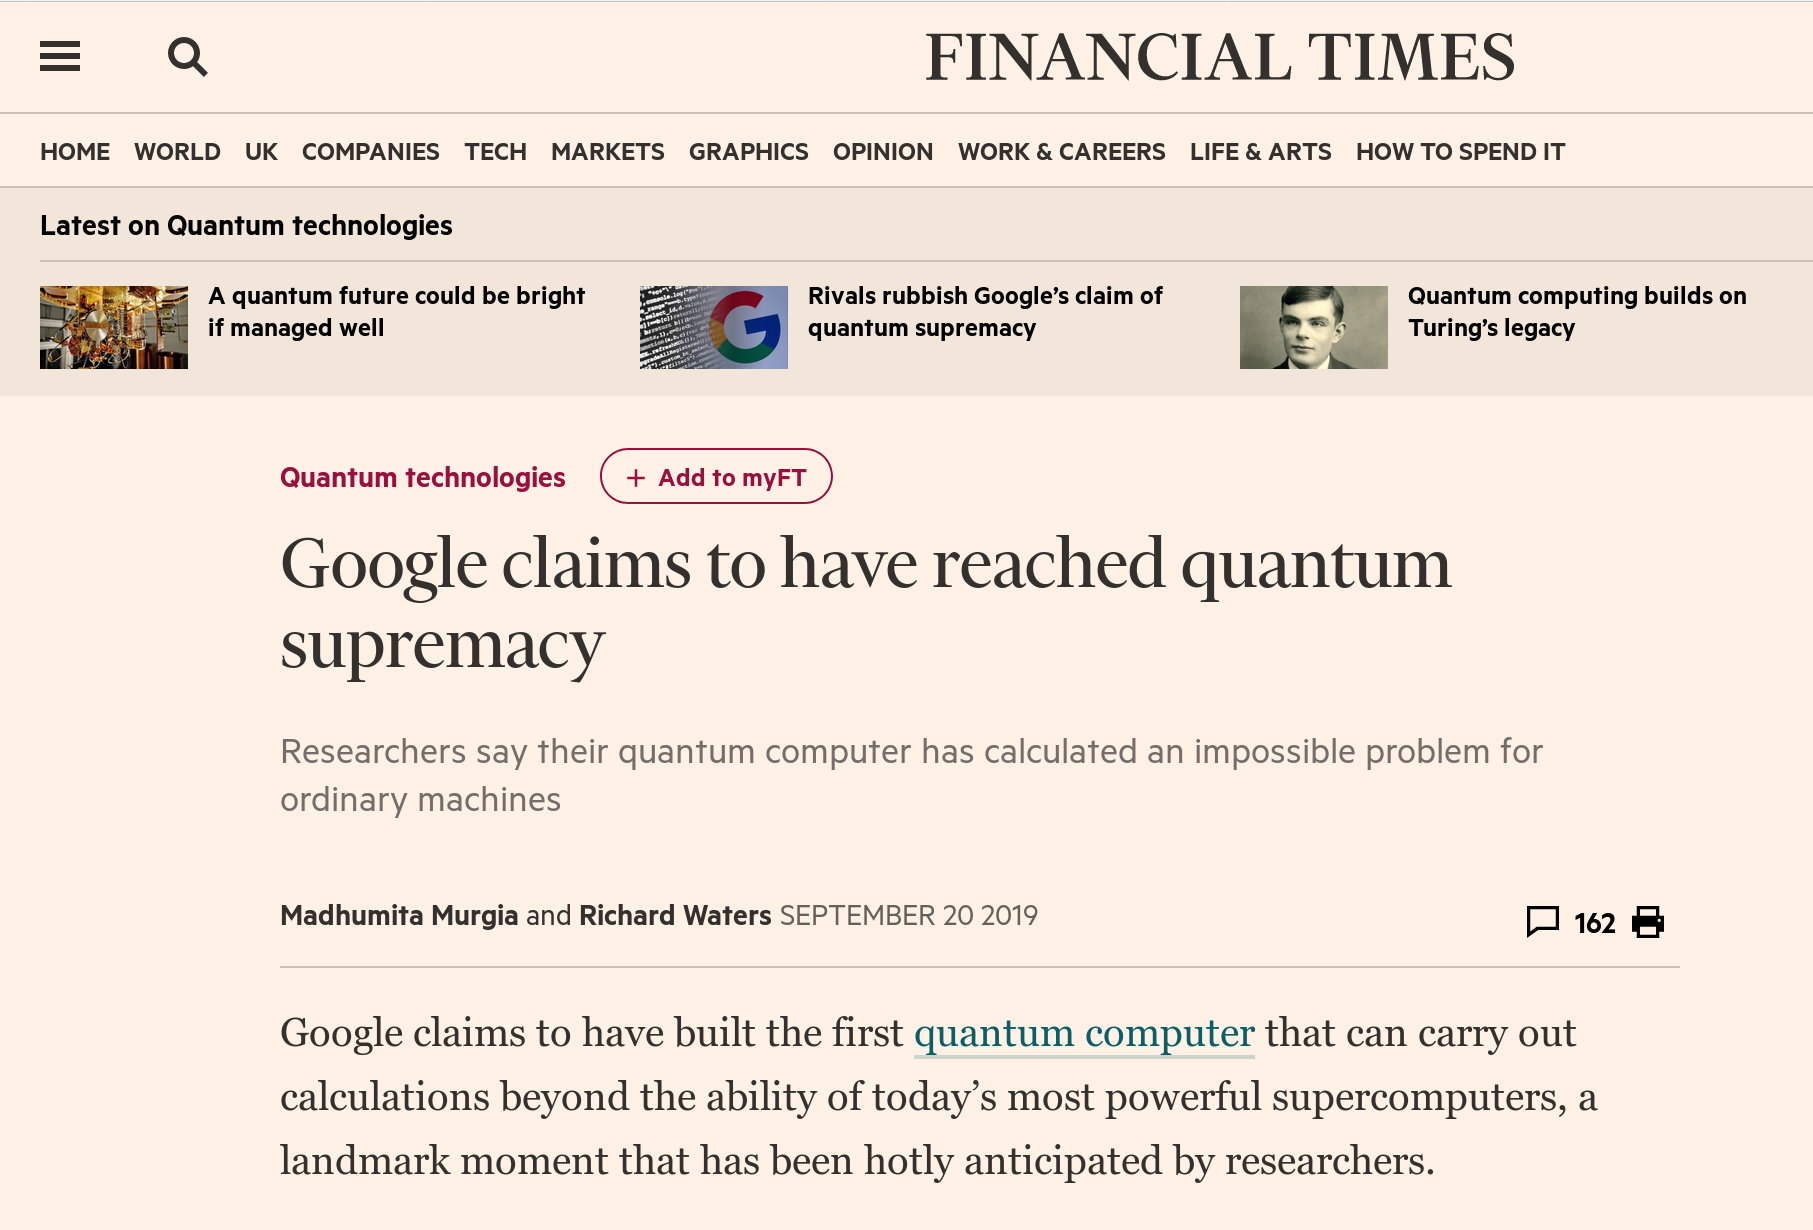
\includegraphics[width=.9\linewidth]{./google-72-qubit.png}
\end{center}
\end{column}
\end{columns}
\end{frame}

\begin{frame}[label={sec:org7c1db6d}]{IBM Quantum Computing Timeline}
\begin{center}
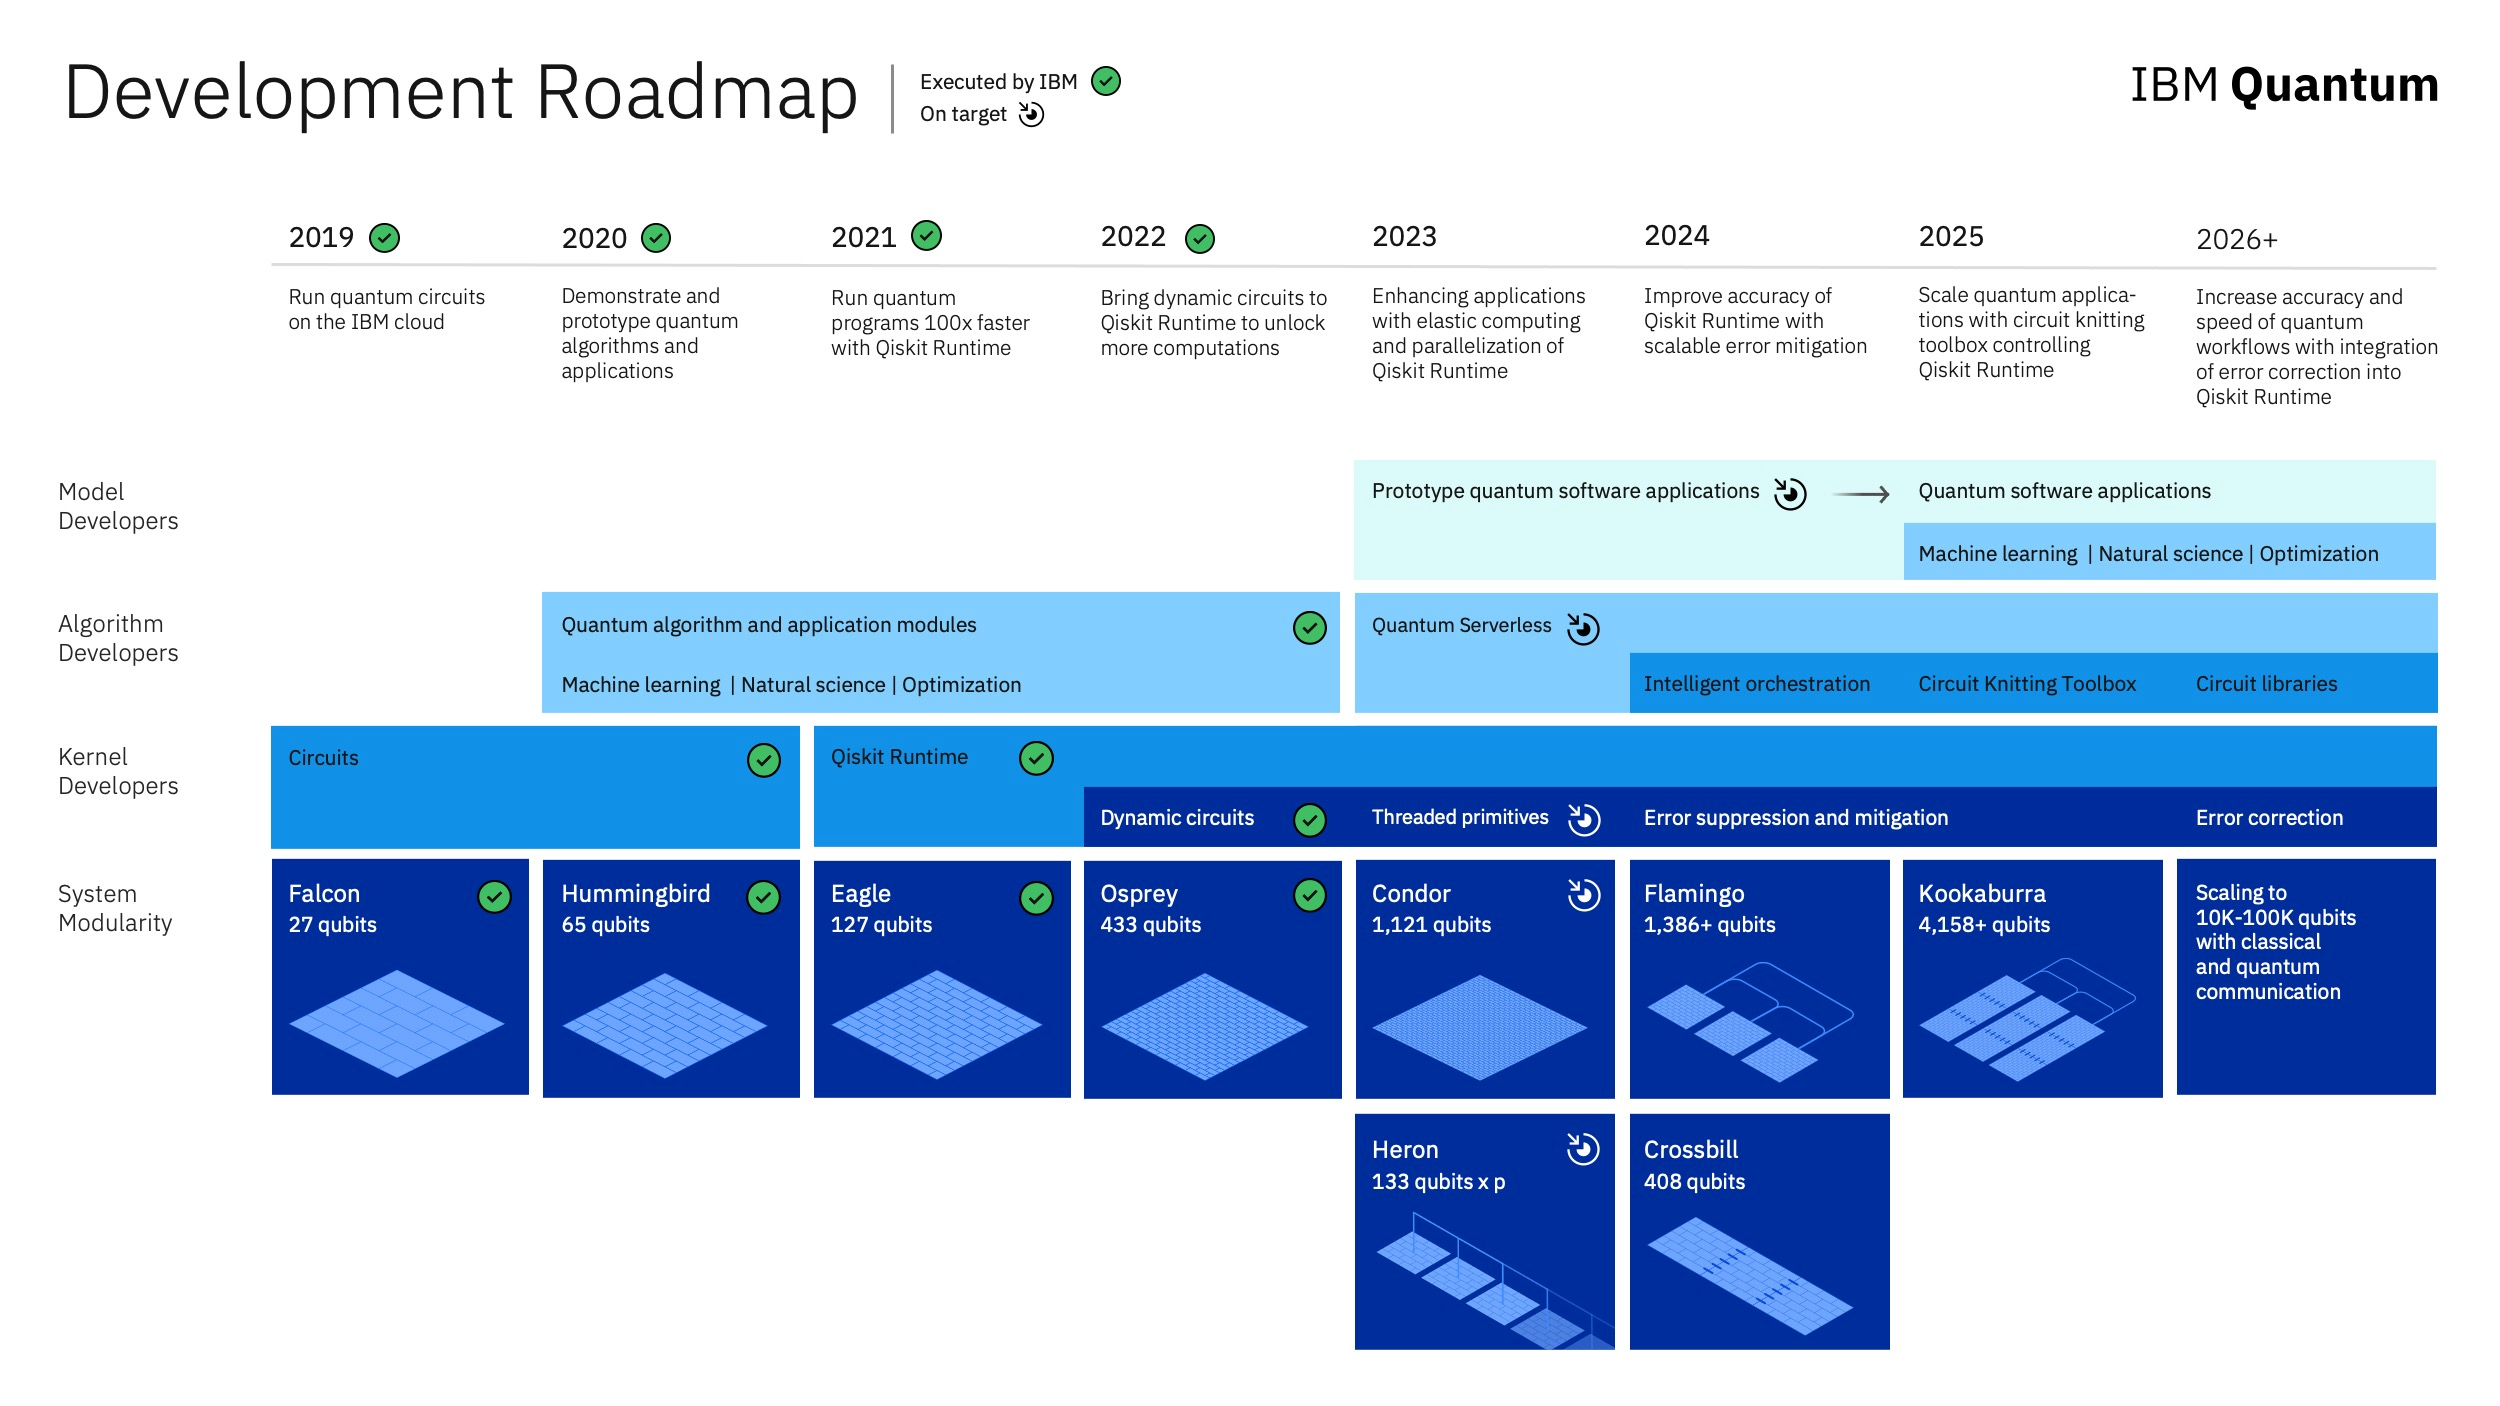
\includegraphics[keepaspectratio,height=.7\textheight]{./IBM-Quantum-DevRoadmap2022_Light.png}
\end{center}

\tiny \url{https://www.ibm.com/quantum/roadmap}
\end{frame}

\begin{frame}[label={sec:orga6ffd91}]{\sout{Quantum Computer Timeline}}
\begin{itemize}
\item NIST PQC Standards are expected some time before end of 2024
\item Other standardisation bodies and authorities will follow suit\footnote{"NCSC guidance for quantum-safe algorithms will follow the outcome of the NIST process by recommending specific algorithms for representative use cases." --- \href{https://www.ncsc.gov.uk/whitepaper/preparing-for-quantum-safe-cryptography}{NCSC: Preparing for Quantum-Safe Cryptography}}
\end{itemize}

\begin{block}{⇒ Post-quantum cryptography is coming regardless of quantum computers}
Do it right: We are ripping out the plumbing, might as well do it right (protocols, formal assurances, etc)
\end{block}
\end{frame}

\begin{frame}[label={sec:orgf3e485e}]{Essential Cryptographic Primitives}
\begin{columns}[t]
\begin{column}{0.5\columnwidth}
\textbf{Symmetric Primitives}

\small

\begin{itemize}
\item Block and stream ciphers (AES, ChaCha20, \ldots)
\item Authentication codes (HMAC, Poly1305, \ldots)
\item Hash functions (SHA-2, SHA-3, \ldots)
\end{itemize}
\end{column}

\begin{column}{0.5\columnwidth}
\textbf{Asymmetric Primitives}

\small

\begin{itemize}
\item Key agreement and public-key encryption (RSA, Diffie-Hellman, ECDH, \ldots)
\item Digital signatures (RSA, DSA, ECDSA, \ldots)
\end{itemize}
\end{column}
\end{columns}

\begin{block}{Applications}
TLS, SSH, banking, smart cards, hard disk encryption …
\end{block}

\vspace{7.2em}
\end{frame}

\begin{frame}[label={sec:org9c7855e}]{Essential Cryptographic Primitives: Theoretical Perspective}
\begin{columns}[t]
\begin{column}{0.5\columnwidth}
\textbf{Minicrypt}

\small

\begin{itemize}
\item Block and stream ciphers
\item Hash functions
\item Authentication codes
\item \textbf{Digital signatures}
\end{itemize}
\end{column}

\begin{column}{0.5\columnwidth}
\textbf{Cryptomania}

\small

\begin{itemize}
\item Key agreement and public-key encryption
\item \ldots
\end{itemize}


\pause
\end{column}
\end{columns}

\begin{block}{Very slow one-time digital signatures from hash functions}
\begin{itemize}
\item \textbf{KeyGen} \(H(\cdot)\) is a hash function with 256 bits of output. Sample random numbers \((a_{0,0}, a_{0,1}), (a_{1,0}, a_{1,1}), \ldots, (a_{255,0}, a_{255,1})\). Publish \(H(a_{i,j})\) for all \(a_{i,j}\).\\[0pt]
\item \textbf{Sign}   Let \(b_i\) be the bits of \(H(m)\). For each bit \(b_i\), publish \(a_{i, b_i}\).\\[0pt]
\item \textbf{Verify} Check that \(a_{i, b_i}\) indeed hashes to \(H(a_{i,j})\) in the public key.
\end{itemize}
\end{block}
\end{frame}

\begin{frame}[label={sec:org73c14c5}]{The Poverty of Public-Key Cryptography}
\begin{columns}[t]
\begin{column}{0.5\columnwidth}
\textbf{Symmetric Primitives}

\phantom{M}

\emph{Indeed, it seems that “you can’t throw a rock without hitting a one-way function” in the sense that, once you cobble together a large number of simple computational operations then, unless the operations satisfy some special property such as linearity, you will typically get a function that is hard to invert}.\footfullcite{EPRINT:Barak17}
\end{column}


\begin{column}{0.5\columnwidth}
\textbf{Asymmetric Primitives}

\phantom{M}

All widely deployed asymmetric cryptography relies on the hardness of 

\textbf{factoring:} \[\textnormal{Given } N = p \cdot q \textnormal{ find } p, \textnormal{ or }\]
\textbf{(elliptic-curve) discrete logarithms:} \[\textnormal{Given }  g^a  \bmod q \textnormal{ and } g \textnormal{ find } a.\]
\end{column}
\end{columns}
\end{frame}

\begin{frame}[label={sec:orgf615b92}]{Symmetric Primitives: Quantum Computing Perspective (Good News)}
Best known quantum algorithms for attacking symmetric cryptography are based on Grover’s algorithm. 

\begin{itemize}
\item Search key space of size \(2^n\) in \(2^{n/2}\) operations: AES-256 \(\rightarrow\) 128 “quantum bits of security”.
\item Taking all costs into account: \(> 2^{152}\) classical operations for AES-256.\footfullcite{EC:JNRV20}
\item Assuming a max depth of \(2^{96}\) for a quantum circuit: overall AES-256 cost is \(\approx 2^{190}\).
\item Does not parallelise: have to wait for \(2^{X}\) steps, cannot buy \(2^{32}\) quantum computers and wait \(2^X / 2^{32}\) steps.
\end{itemize}
\end{frame}

\begin{frame}[label={sec:org08c0987}]{Asymmetric Primitives: Quantum Computing Perspective}
\begin{center}
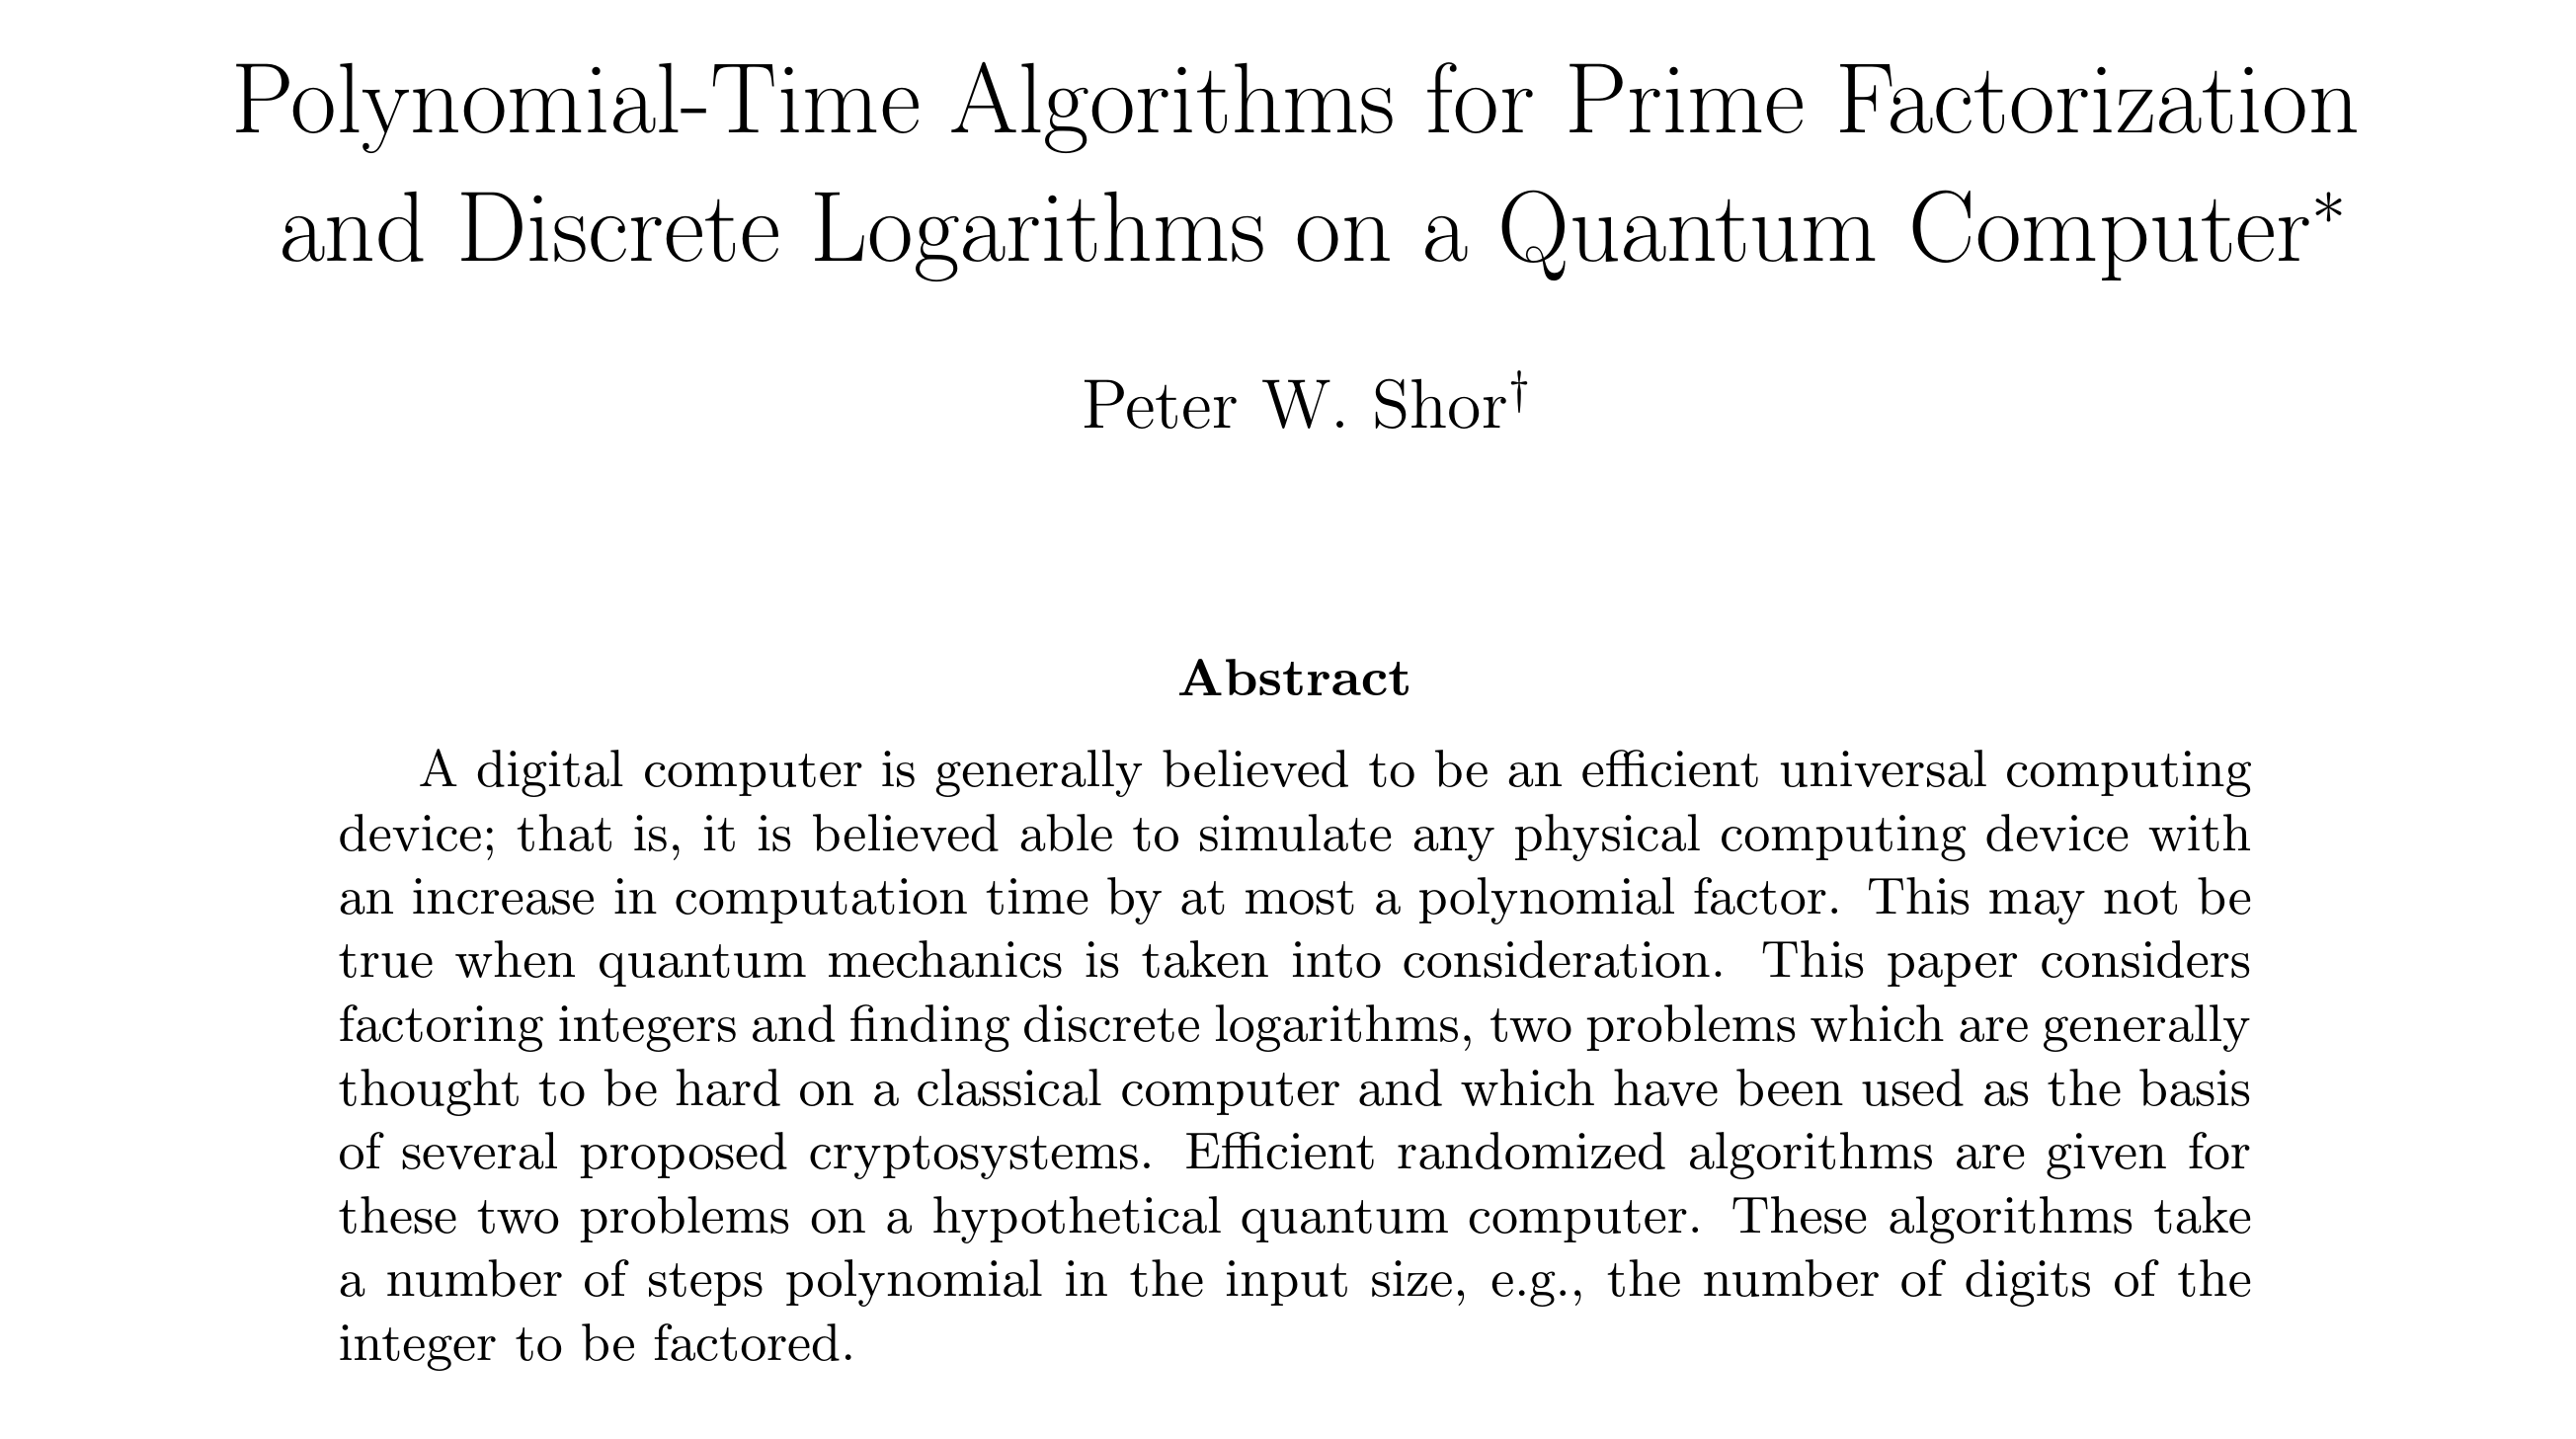
\includegraphics[width=.9\linewidth]{./shor.png}
\end{center}
\end{frame}

\begin{frame}[label={sec:org29b8672}]{Asymmetric Primitives: Quantum Computing Perspective}
\begin{center}
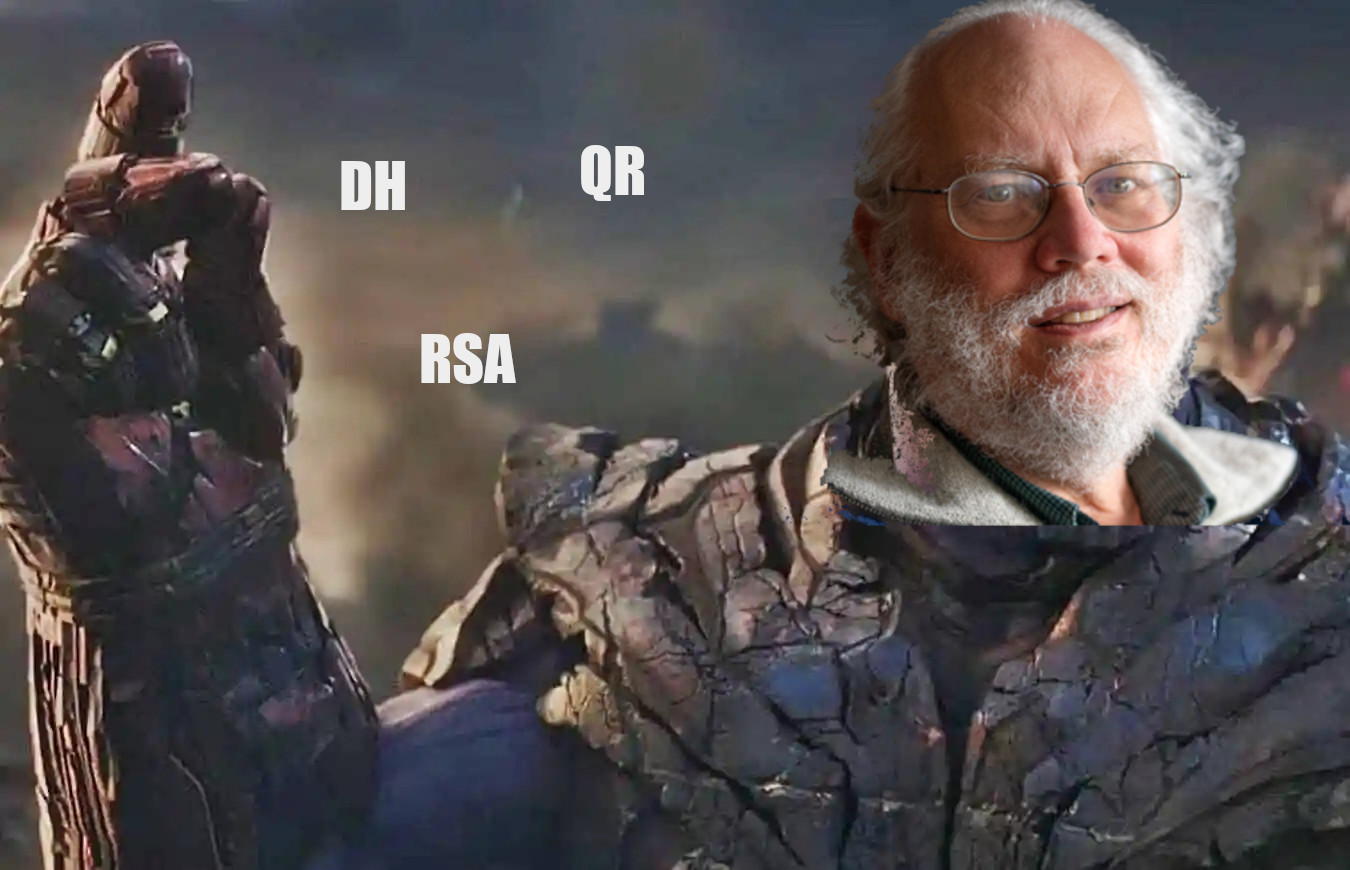
\includegraphics[keepaspectratio,width=.9\linewidth,height=.9\textheight]{./shor-2.jpeg}
\end{center}
\end{frame}

\section{Post-Quantum Standardisation}
\label{sec:org5607675}
\begin{frame}[label={sec:org9504c8a}]{Post-Quantum Standardisation}
\begin{description}
\item[{NIST}] \textbf{Post Quantum \sout{Competition} Process}
\item[{ETSI}] Cyber Working Group for Quantum Safe Cryptography
\item[{ISO}] WG2 Standing Document 8 (SD8): Survey
\item[{IETF}] Standardisation of \textbf{stateful} hash-based signatures, nothing further
\item[{CSA}] Quantum-safe Security Working Group: position papers
\item[{NIST}] \textbf{Post Quantum Process: Digital Signatures}
\end{description}

\pause

\begin{alertblock}{Bottom Line}
Essentially, everyone is/was waiting for NIST.
\end{alertblock}

\vspace{0.7em}
\end{frame}
\begin{frame}[label={sec:org08351e5},fragile]{NIST PQC \sout{Competition} Process}
 \textbf{Timeline}

\begin{center}
\begin{tabular}{ll}
\toprule
Submission & November 2017\\[0pt]
Round 2 Selection & January 2019\\[0pt]
Round 3 Selection & July 2020\\[0pt]
Winners and Round 4 Selection & July 2022\\[0pt]
Final Standard Expectation & by 2024\\[0pt]
\bottomrule
\end{tabular}

\end{center}

\vspace{1em}

\begin{columns}[t]
\begin{column}{0.5\columnwidth}
\textbf{“Key Establishment”/Key Encapsulation}

\begin{itemize}
\item \texttt{(pk,sk) ← KeyGen()}
\item \texttt{(c,k) ← Encaps(pk)}
\item \texttt{k ← Decaps(c,sk)}
\end{itemize}
\end{column}

\begin{column}{0.5\columnwidth}
\textbf{Digital Signature}

\begin{itemize}
\item \texttt{(vk,sk)  ← KeyGen()}
\item \texttt{s  ← Sig(m,sk)}
\item \texttt{\{0,1\}  ← Verify(s,m,vk)}
\end{itemize}
\end{column}
\end{columns}
\end{frame}
\begin{frame}[label={sec:org81699ff},fragile]{KEM: Security}
 \begin{columns}[t]
\begin{column}{0.5\columnwidth}
\textbf{What you get: "IND-CCA"}

\begin{itemize}
\item We give the adversary either the real \texttt{k} or a random fake one.
\item The adversary is allowed to ask for decryptions of \alert{any} ciphertext but \texttt{c}
\item The adversary wins if it guesses correctly which key we gave it
\end{itemize}

This implies the adversary cannot learn anything about an encrypted message (except its length) even when being allowed to decrypt anything else.
\end{column}

\begin{column}{0.5\columnwidth}
\textbf{What you \emph{do not} get}

\begin{itemize}
\item Given a ciphertext it is unclear who it was encrypted too
\begin{itemize}
\item Ciphertexts might reveal what keys can decrypt them
\end{itemize}
\item If you can decrypt, only you can decrypt
\begin{itemize}
\item It might be possible construct a ciphertext that decrypts correctly under two or more decryption keys
\end{itemize}
\item …
\end{itemize}
\end{column}
\end{columns}
\end{frame}

\begin{frame}[label={sec:org88a07d3}]{KEM: Kyber}
\begin{columns}[t]
\begin{column}{0.5\columnwidth}
\textbf{RSA 2048}

\begin{center}
\begin{tabular}{lr}
\toprule
Key generation & \(\approx\) 130,000,000 cycles\\[0pt]
Encapsulation & \(\approx\) 20,000 cycles\\[0pt]
Decapsulation & \(\approx\) 2,700,000 cycles\\[0pt]
Ciphertext & 256 bytes\\[0pt]
Public key & 256 bytes\\[0pt]
\bottomrule
\end{tabular}

\end{center}

{\tiny \url{https://bench.cr.yp.to/results-kem.html} }

\textbf{Curve25519}

\begin{center}
\begin{tabular}{lr}
\toprule
Key generation & \(\approx\) 60,000 cycles\\[0pt]
Key agreement & \(\approx\) 160,000 cycles\\[0pt]
 & \\[0pt]
Public key & 32 bytes\\[0pt]
Key Share & 32 bytes\\[0pt]
\bottomrule
\end{tabular}

\end{center}

\tiny \url{https://eprint.iacr.org/2015/943}
\end{column}

\begin{column}{0.5\columnwidth}
\textbf{Kyber-768}

\begin{center}
\begin{tabular}{lr}
\toprule
Key generation & ≈  38,000 cycles\\[0pt]
Encapsulation & ≈  49,000 cycles\\[0pt]
Decapsulation & ≈  39,000 cycles\\[0pt]
Ciphertext & 1,088 bytes\\[0pt]
Public key & 1,184 bytes\\[0pt]
\bottomrule
\end{tabular}

\end{center}

\tiny \url{https://bench.cr.yp.to/results-kem.html}
\end{column}
\end{columns}
\end{frame}
\begin{frame}[label={sec:orga8ab36e},fragile]{Lattice-based KEM: Learning with Errors}
 \textbf{"KeyGen:"}

\begin{lstlisting}[language=Python,label= ,caption= ,captionpos=b,numbers=none]
A = random_matrix(GF(7681), 3*256, 3*256)
s = random_vector(ZZ, 3*256, x=-4, y=5)
\end{lstlisting}

\textbf{"Encrypt:"}

\begin{lstlisting}[language=Python,label= ,caption= ,captionpos=b,numbers=none]
e = random_vector(ZZ, 3*256, x=-4, y=5) # this makes it hard!
m = random_vector(GF(2), 3*256).lift()
b = A*s + e + 7681//2 * m # encrypt
\end{lstlisting}

\textbf{"Decrypt:"}

\begin{lstlisting}[language=Python,label= ,caption= ,captionpos=b,numbers=none]
r = (b - A*s).lift_centered() # this is == e + 7681//2 * m
vector(ZZ, [round(float(r_)/(7681//2)) for r_ in r]) == m # round and check
\end{lstlisting}

\begin{verbatim}
True
\end{verbatim}
\end{frame}

\begin{frame}[label={sec:org74f555d}]{SIG: Security}
\begin{columns}[t]
\begin{column}{0.5\columnwidth}
\textbf{What you get: "EUF-CMA"}

\begin{itemize}
\item An adversary is allowed to ask us to sign any message it wants, as often as it likes
\item The adversary wins if it then outputs a valid signature for a message \alert{it has not asked us for a signature before}
\item A valid signature is a signature that checks out \alert{given} the verification key.
\end{itemize}
\end{column}

\begin{column}{0.5\columnwidth}
\textbf{What you \emph{do not} get}

\begin{itemize}
\item Given a signature and it verifies under a given verification key then it was signed by the matching sender
\begin{itemize}
\item There might be more than one verification key under which a signature validates
\end{itemize}
\item Given a signature and message pair, there is only this one message for a given signature.
\begin{itemize}
\item The same signature might be valid for multiple messages.
\end{itemize}
\item …
\end{itemize}
\end{column}
\end{columns}
\end{frame}

\begin{frame}[label={sec:org91d65f4}]{SIG: Lattic-based (Falcon, Dilithium) or Hash-based (SPHINCS+)}
\begin{center}
\begin{tabular}{lrrrr}
\toprule
Scheme & PK & Sig & Verif & Sign\\[0pt]
\midrule
NIST P-256 & 64 & 64 & 1 (baseline) & 1 (baseline)\\[0pt]
RSA-2048 & 256 & 256 & 0.2 & 25\\[0pt]
\midrule
Dilithium2 & 1,320 & 2,420 & 0.3 & 2.5\\[0pt]
Falcon-512 & 897 & 666 & 0.3 & 5\\[0pt]
Falcon-512 FPEMU & 897 & 666 & 0.3 & 100\\[0pt]
SPHINCS+-128ss har. & 32 & 7,856 & 1.7 & 3,000\\[0pt]
\bottomrule
\end{tabular}

\end{center}

\tiny \url{https://blog.cloudflare.com/sizing-up-post-quantum-signatures/}
\end{frame}

\begin{frame}[label={sec:orgd88c94a},fragile]{Lattice-based SIG: Short Integer Solutions}
 \textbf{Easy:}

\begin{lstlisting}[language=Python,label= ,caption= ,captionpos=b,numbers=none]
q = next_prime(2^13)
A = random_matrix(GF(q), 1024, 2048)
u = random_vector(ZZ, 2048, x=-ceil(sqrt(q)), y=ceil(sqrt(q)))
t = A*u # easy
assert max(u) < q//4 
\end{lstlisting}

\textbf{Hard:}

\begin{lstlisting}[language=Python,label= ,caption= ,captionpos=b,numbers=none]
v = A.solve_right(t).lift_centered()
assert A*v == t
max(v) < q//4
\end{lstlisting}

\begin{verbatim}
False
\end{verbatim}
\end{frame}

\section{Post-Quantum Security}
\label{sec:org14ed2c0}
\begin{frame}[label={sec:org41c3a13},fragile]{Security Notions}
 \begin{description}
\item[{KEM}] \textbf{IND-CCA}: Given some challenge ciphertext \texttt{c} and some key \texttt{k}, the adversary gets an oracle to decapsulate (“decrypt”) any other ciphertext but still cannot decide if \texttt{c} encapsulates (“encrypts”) the key \texttt{k}.

\item[{SIG}] \textbf{EUF-CMA}: Given access to some oracle that signs arbitrary messages, the adversary still cannot produce a valid signature of a message not previously submitted to the signing oracle.
\end{description}

\pause

\begin{block}{Computational Security}
“cannot“ \(\rightarrow\) “it takes too long even given access to a quantum computer.”


\pause
\end{block}

\begin{block}{Conditional Security}
“cannot” \(\rightarrow\) “… assuming some mathematical problem is hard on a quantum computer”
\end{block}
\end{frame}

\begin{frame}[label={sec:org4082e51}]{SIKE Attack}
\fullcite{EPRINT:CasDec22}

\begin{itemize}
\item SIDH was “A decade unscathed” \cite{EPRINT:Costello21}
\item SIKE even \emph{lowered} parameters during NIST PQC (following \cite{C:JaqSch19})
\item qualified researchers tried to break it (e.g. \cite{EPRINT:MarPan19})
\end{itemize}

\begin{alertblock}{Total Break}
All SIKE parameters can be broken in about 2 hours on a single-core laptop now \cite{EPRINT:OudPop22}.
\end{alertblock}
\end{frame}
\begin{frame}[label={sec:org9d5ca36}]{Rainbow Attack}
\begin{columns}[t]
\begin{column}{0.6\columnwidth}
\begin{center}
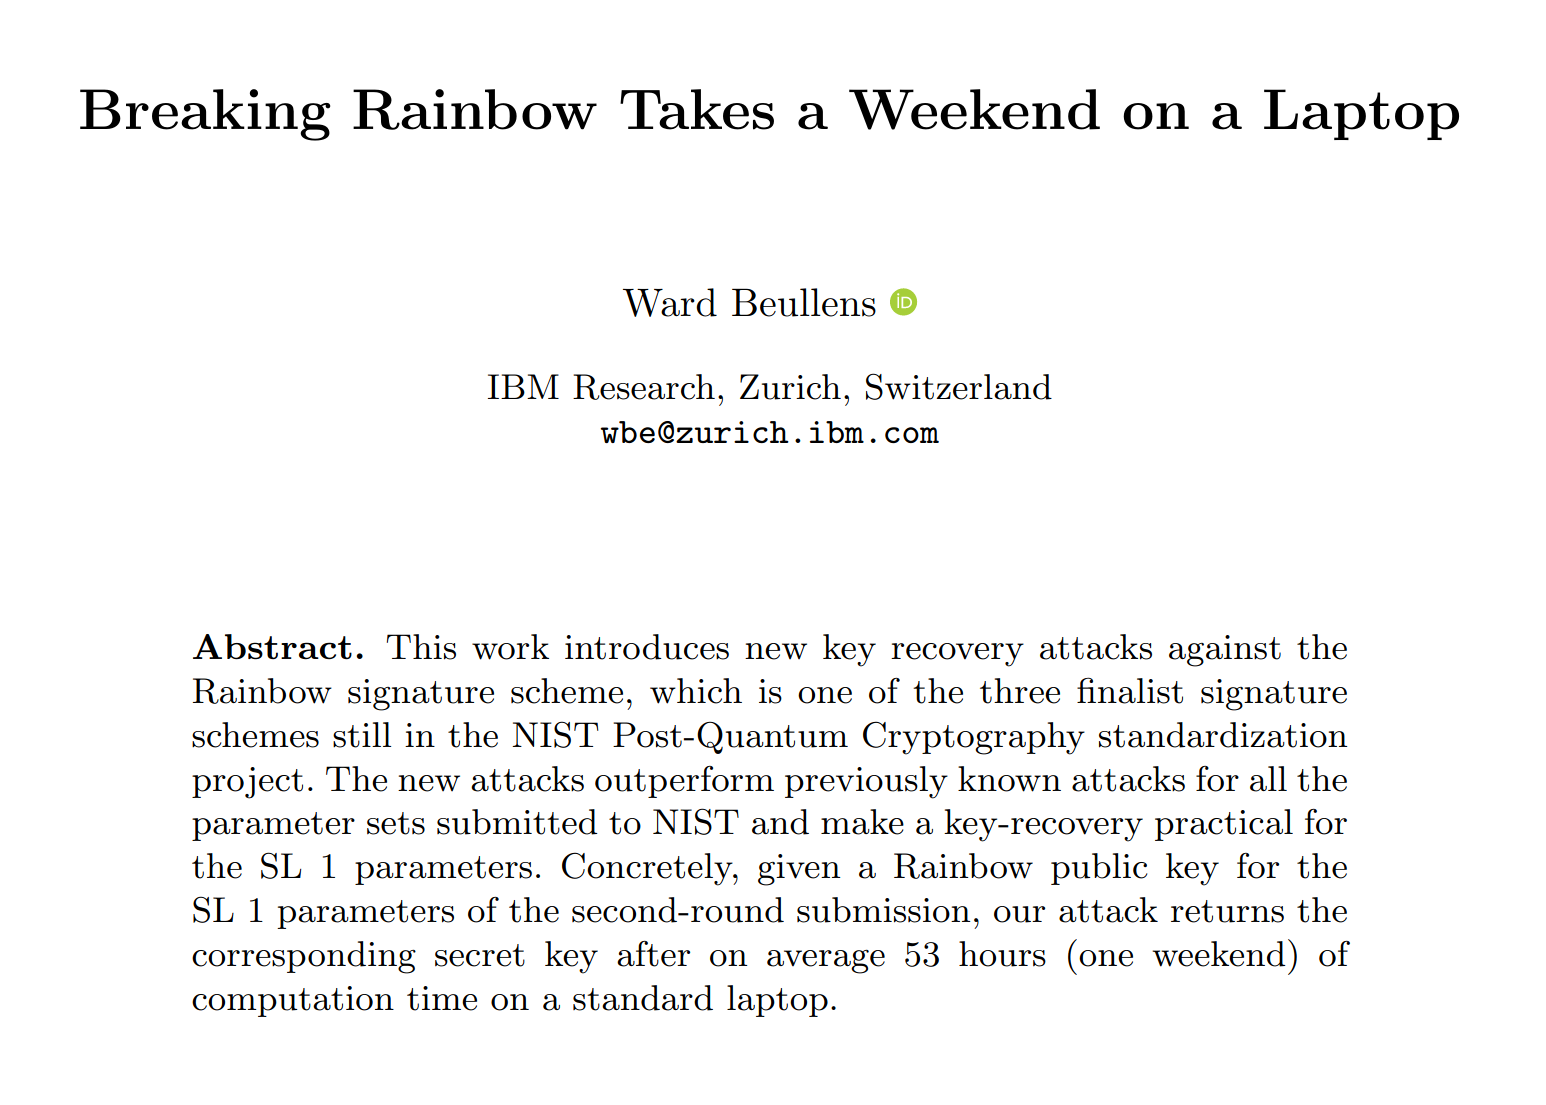
\includegraphics[keepaspectratio,height=.8\textheight]{./breaking-rainbow.png}
\end{center}
\end{column}

\begin{column}{0.4\columnwidth}
\begin{itemize}
\item Rainbow was a NIST finalist \cite{EPRINT:Beullens22}
\item Can be remedied by increasing parameters
\item MQ signatures have a shaky history
\item NIST is specifically looking to standardise UOV, a long-standing MQ signature scheme
\end{itemize}
\end{column}
\end{columns}
\end{frame}
\begin{frame}[label={sec:org5169910}]{MATZOV Attack}
\begin{columns}[t]
\begin{column}{0.6\columnwidth}
\begin{center}
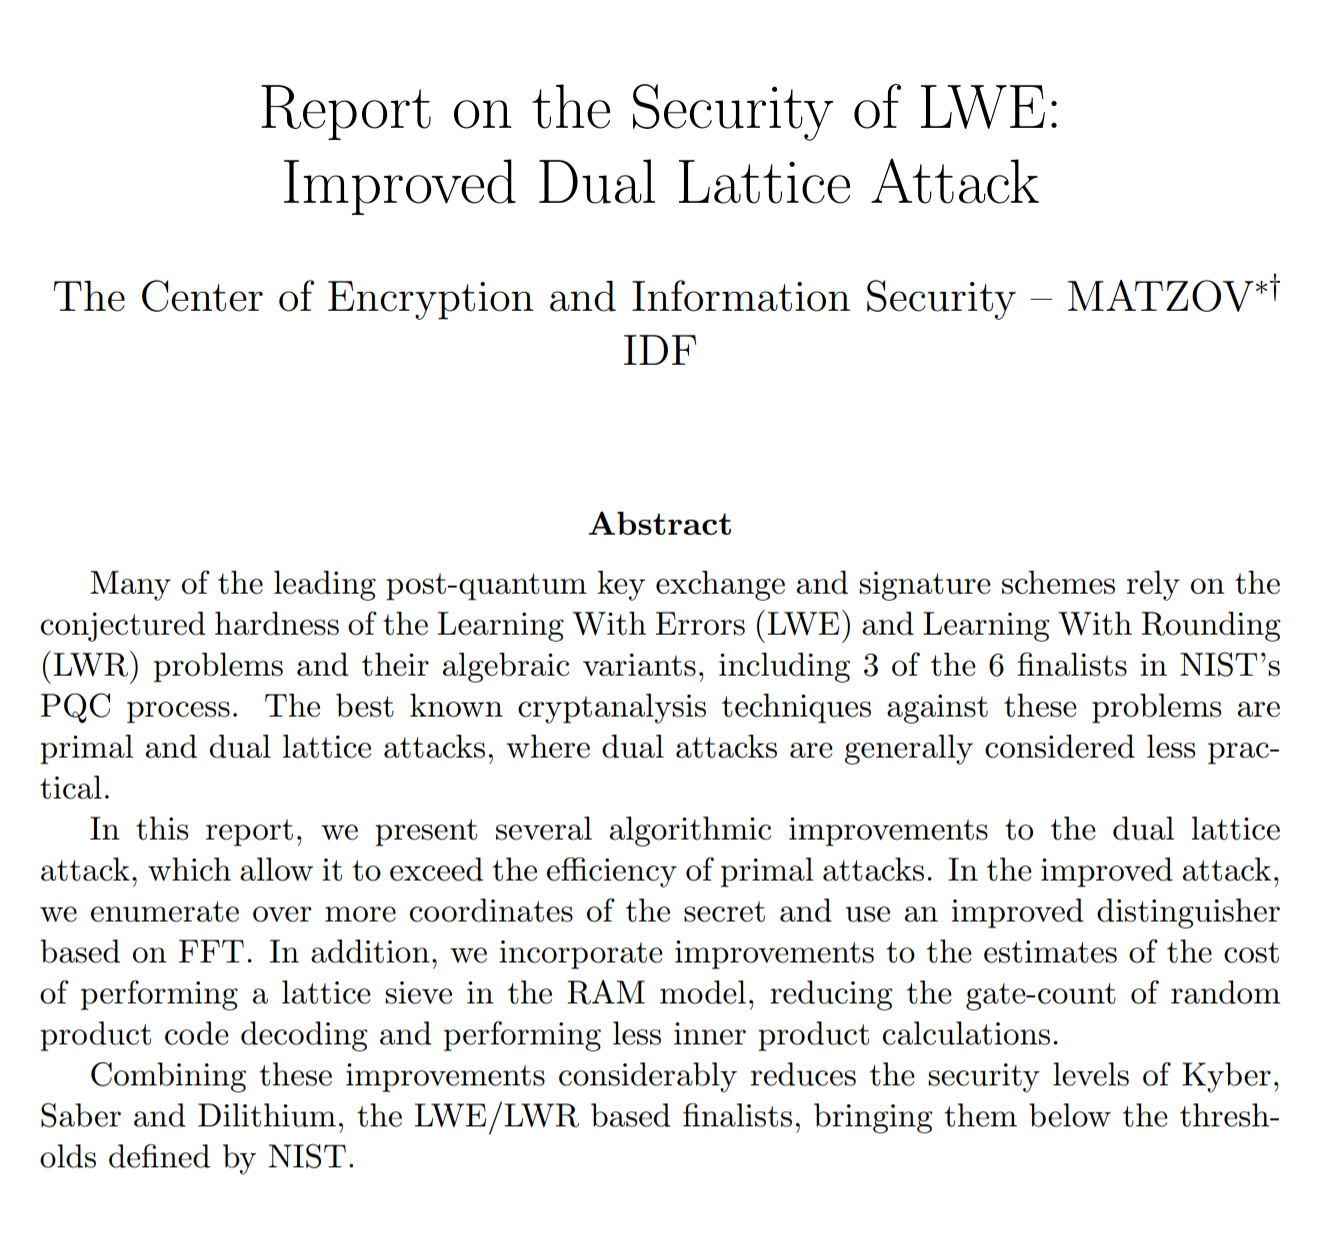
\includegraphics[keepaspectratio,height=.8\textheight]{./matzov.png}
\end{center}
\end{column}

\begin{column}{0.4\columnwidth}
\begin{itemize}
\item Made some waves, partly due to the authorship
\item Ingredients:
\begin{itemize}
\item Improvement in a lower-order "sieving" term
\item Generalisation of a technique from \cite{AC:GuoJoh21}
\end{itemize}
\item Precise impact a bit unclear \footfullcite{EPRINT:DucPul23}
\end{itemize}
\end{column}
\end{columns}
\end{frame}

\begin{frame}[label={sec:orgfb24544}]{Lattices}
\(\frac{3}{4}\) selected NIST algorithms are based on structured lattices

\begin{itemize}
\item We have good evidence that lattice problems are hard asymptotically.
\item We have a relatively good understanding of how know algorithms behave concretely.
\begin{itemize}
\item Our estimates are conservative, ignoring e.g. the cost of memory access.
\end{itemize}
\item Quantum computers seem to not help for lattices in any meaningful way.
\item No known algorithms that perform better on structured lattices than on unstructured lattices.
\begin{itemize}
\item Biggest potential for improvements here!
\end{itemize}
\end{itemize}
\end{frame}
\section{Post-Quantum Hedging}
\label{sec:org5072443}
\begin{frame}[label={sec:orgba6c9f7}]{NIST Round 4}
\begin{columns}
\begin{column}{0.3\columnwidth}
\begin{itemize}
\item BIKE
\item Classic McEliece
\item HQC
\item {\color{lightgray}{SIKE}}\footnote{See above.}
\end{itemize}
\end{column}

\begin{column}{0.7\columnwidth}
"Both BIKE and HQC are based on structured codes, and either would be suitable as a general-purpose KEM that is not based on lattices. NIST expects to select at most one of these two candidates for standardization at the conclusion of the fourth round. (…)

Classic McEliece was a finalist but is not being standardized by NIST at this time. Although Classic McEliece is widely regarded as secure, NIST does not anticipate it being widely used due to its large public key size. NIST may choose to standardize Classic McEliece at the end of the fourth round."
\end{column}
\end{columns}
\end{frame}

\begin{frame}[label={sec:orge7fefda}]{Hybrids}
\begin{columns}[t]
\begin{column}{0.3\columnwidth}
\begin{center}

\includegraphics[keepaspectratio,height=0.6\textheight]{./drake.jpg}
\end{center}
\end{column}

\begin{column}{0.7\columnwidth}
\begin{center}
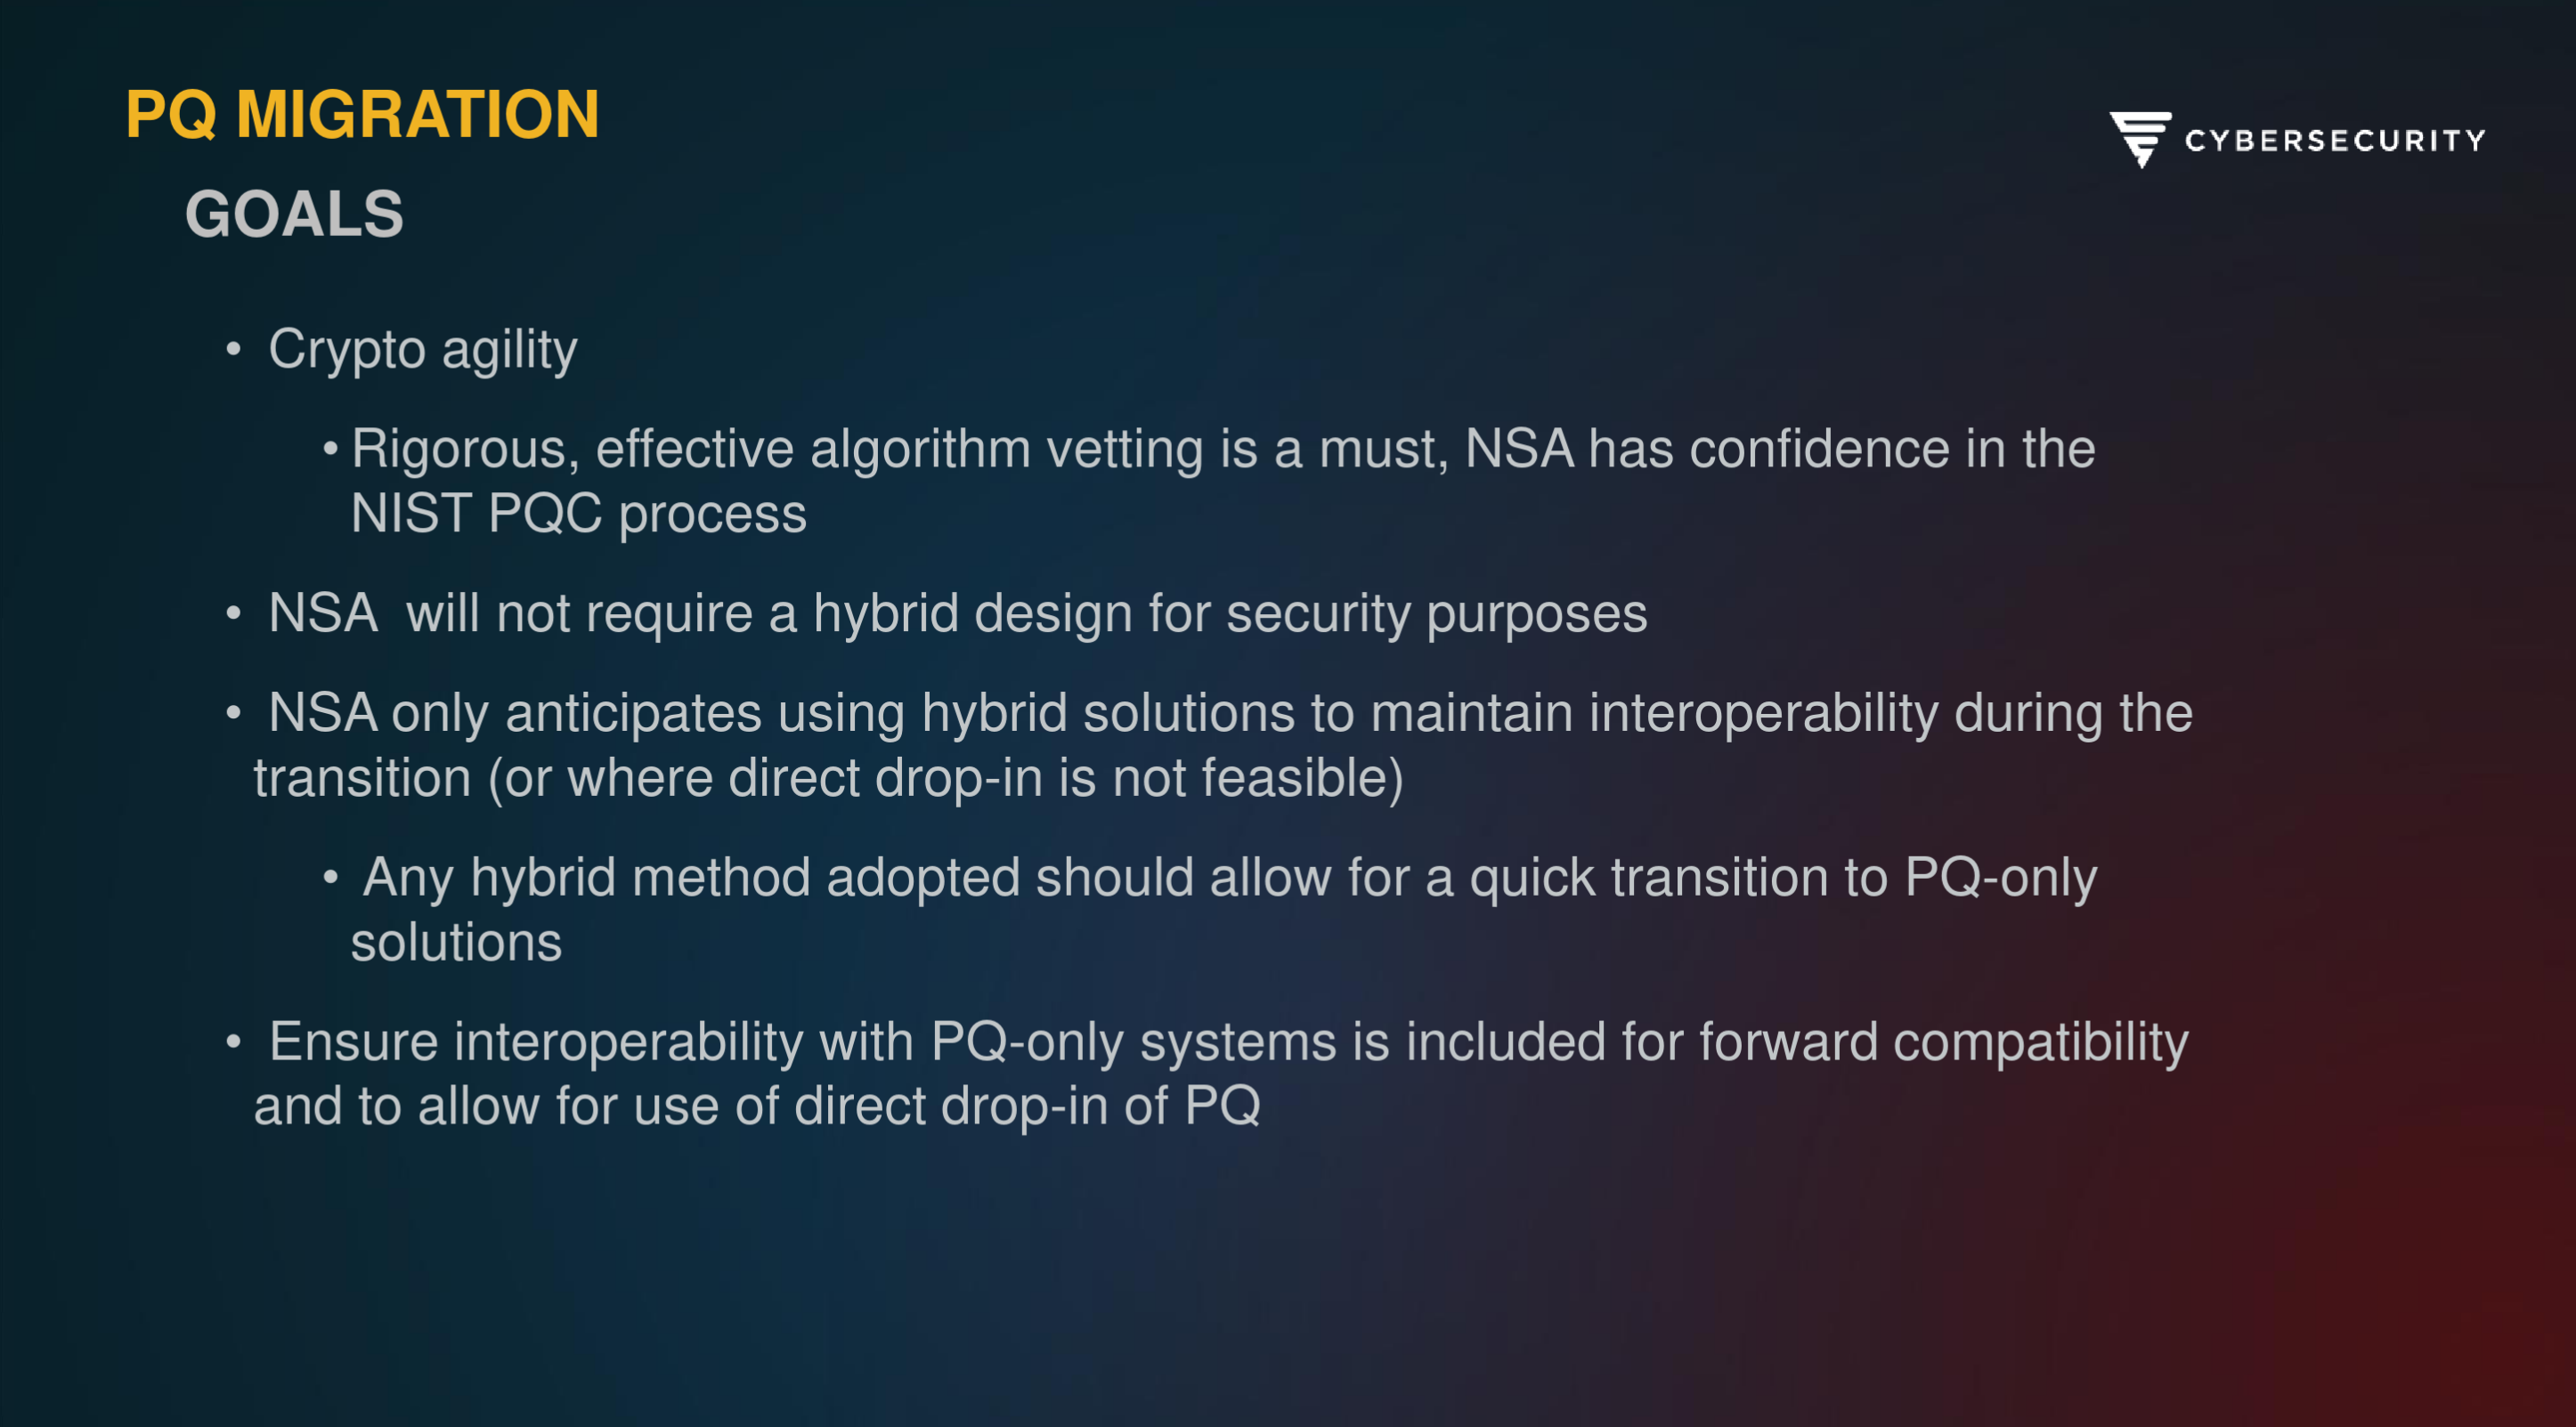
\includegraphics[keepaspectratio,height=0.6\textheight]{./nsa-be-like.png}
\end{center}

\tiny \url{https://datatracker.ietf.org/meeting/112/materials/slides-112-lamps-hybrid-non-composite-multi-certificate-00}
\end{column}
\end{columns}

\begin{alertblock}{Other Agencies}
\href{https://www.bsi.bund.de/EN/Themen/Unternehmen-und-Organisationen/Informationen-und-Empfehlungen/Quantentechnologien-und-Post-Quanten-Kryptografie/quantentechnologien-und-post-quanten-kryptografie\_node.html}{BSI} (Germany) and \href{https://www.ssi.gouv.fr/en/publication/anssi-views-on-the-post-quantum-cryptography-transition/}{ANSSI} (France) recommend hybrid encryption.
\end{alertblock}
\end{frame}
\begin{frame}[label={sec:orga53e988}]{NIST Digital Signatures}
\begin{quote}
"NIST also plans to issue a new Call for Proposals for public-key (quantum-resistant) digital signature algorithms by the end of summer 2022. NIST is primarily looking to diversify its signature portfolio, so signature schemes that are \textbf{not based on structured lattices} are of greatest interest. NIST would like submissions for signature schemes that have short signatures and fast verification (e.g., \textbf{UOV})." --- Dustin Moody (NIST) on \href{https://groups.google.com/a/list.nist.gov/g/pqc-forum/c/G0DoD7lkGPk/m/f3Hl0sh3AgAJ}{PQC mailinglist}, my emphasis
\end{quote}
\end{frame}

\begin{frame}[label={sec:org1fbc2a3}]{NIST Digital Signature Submissions}
\begin{columns}[t]
\begin{column}{0.4\columnwidth}
\begin{itemize}
\item \alert<1>{Lattices}
\item \alert<2>{Codes}
\item \alert<3>{MPC-in-the-Head}
\item \alert<4>{Multivariate}
\item \alert<5>{Isogenies}
\item \alert<6>{Symmetric}
\item \alert<7>{Other}
\end{itemize}
\end{column}

\begin{column}{0.6\columnwidth}
\textbf{40 Submissions}

\alert<4>{3WISE},
\alert<6>{AIMer},
\alert<7>{ALTEQ},
\alert<6>{Ascon-Sign},
\alert<4>{Biscuit},
\alert<3>{CROSS},
\alert<4>{DME-Sign},
\alert<1>{EHT},
\alert<1>{EagleSign},
\alert<2>{Enhanced pqsigRM},
\alert<6>{FAEST},
\alert<2>{FuLeeca},
\alert<1>{HAETAE},
\alert<1>{HAWK},
\alert<4>{HPPC},
\alert<1>{HuFu},
\alert<7>{KAZ-SIGN},
\alert<2>{LESS},
\alert<4>{MAYO},
\alert<2>{MEDS},
\alert<3>{MIRA},
\alert<3>{MQOM},
\alert<3>{MiRitH},
\alert<3>{PERK},
\alert<4>{PROV},
\alert<7>{Preon},
\alert<4>{QR-UOV},
\alert<3>{RYDE},
\alert<1>{Raccoon},
\alert<3>{SDitH},
\alert<4>{SNOVA},
\alert<6>{SPHINCS-alpha},
\alert<5>{SQIsign},
\alert<1>{SQUIRRELS},
\alert<4>{TUOV},
\alert<4>{UOV},
\alert<4>{VOX},
\alert<2>{Wave},
\alert<7>{Xifrat1-Sign.I},
\alert<7>{eMLE-Sig 2.0}
\end{column}
\end{columns}
\end{frame}

\begin{frame}[label={sec:org21b60b2}]{Performance}
\begin{center}
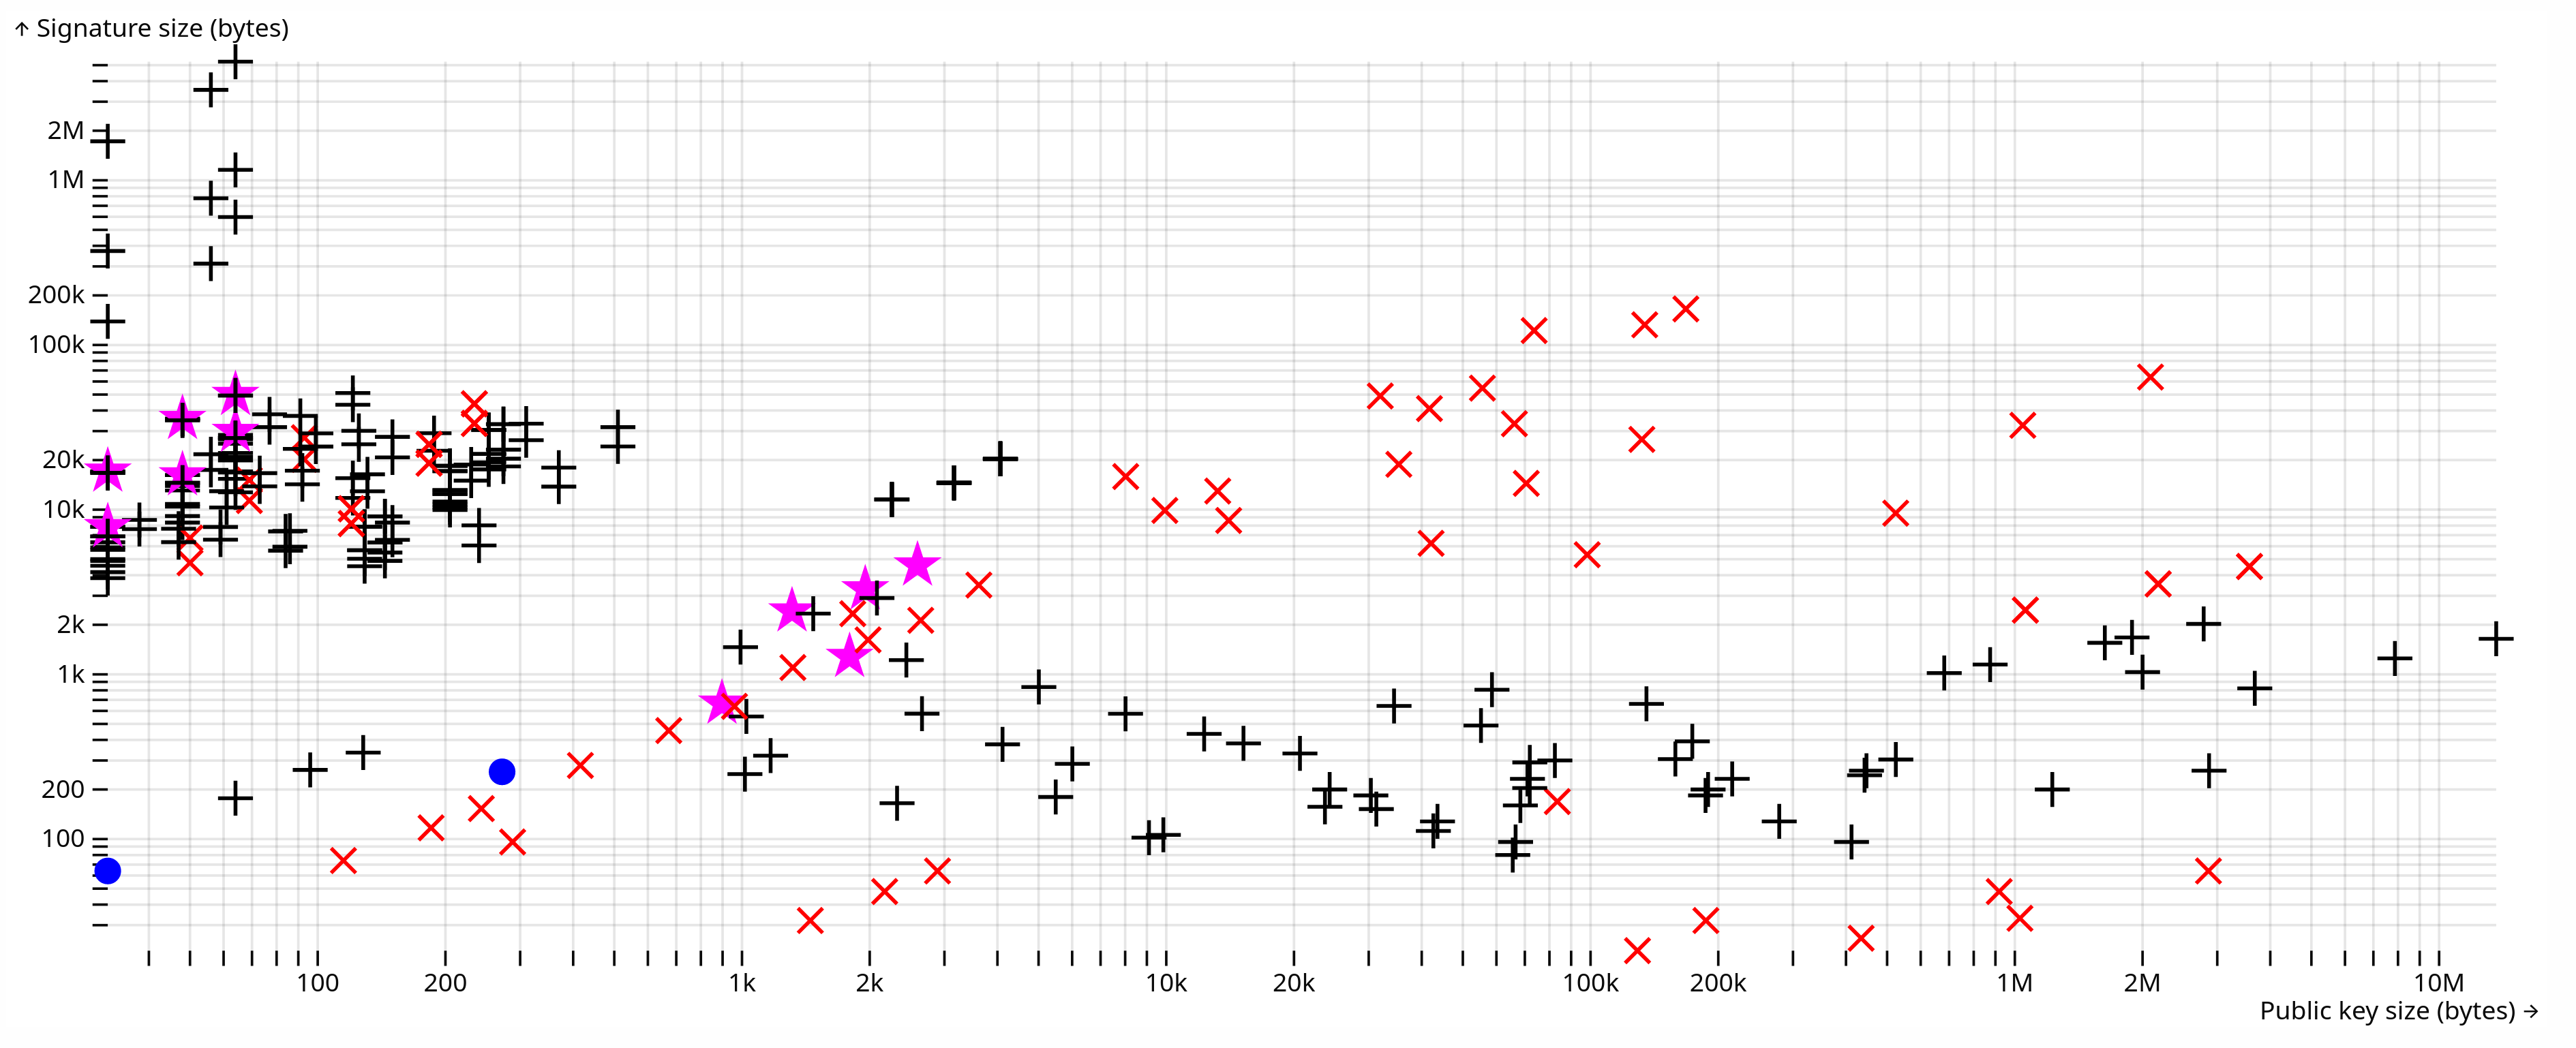
\includegraphics[width=.9\linewidth]{./pqc-signatures.png}
\end{center}

\tiny source: \url{https://pqshield.github.io/nist-sigs-zoo/wide.html}
\end{frame}

\begin{frame}[label={sec:orgd52e26d}]{Vulnerabilities in Specification}
\alert{3WISE},\footnote{\url{https://groups.google.com/a/list.nist.gov/g/pqc-forum/c/fsfGqHCgGvY}}
AIMer,
ALTEQ,
Ascon-Sign,
\alert{Biscuit},\footnote{\url{https://groups.google.com/a/list.nist.gov/g/pqc-forum/c/sw8NueiNek0}}
CROSS,
\alert{DME-Sign},\footnote{\url{https://groups.google.com/a/list.nist.gov/g/pqc-forum/c/E0mMMGI5eWE}}
\alert{EHT},\footnote{\url{https://groups.google.com/a/list.nist.gov/g/pqc-forum/c/mFl\_5Rq6-RU}}
\alert{EagleSign},\footnote{\url{https://groups.google.com/a/list.nist.gov/g/pqc-forum/c/zas5PLiBe6A}}
\alert{Enhanced pqsigRM},\footnote{\url{https://groups.google.com/a/list.nist.gov/g/pqc-forum/c/yQ1CKOLbGng}}
FAEST,
\alert{FuLeeca},\footnote{\url{https://groups.google.com/a/list.nist.gov/g/pqc-forum/c/KvIege2EbuM}}
HAETAE,
HAWK,
\alert{HPPC},\footnote{\url{https://groups.google.com/a/list.nist.gov/g/pqc-forum/c/KRh8w03PW4E}}
\alert{HuFu},\footnote{\url{https://groups.google.com/a/list.nist.gov/g/pqc-forum/c/Hq-wRFDbIaU}}
\alert{KAZ-SIGN},\footnote{\url{https://groups.google.com/a/list.nist.gov/g/pqc-forum/c/aCbi4BMDeUs}}
\alert{LESS},\footnote{\url{https://groups.google.com/a/list.nist.gov/g/pqc-forum/c/Z36SPZJI8Ok}}
MAYO,
\alert{MEDS},\footnote{\url{https://groups.google.com/a/list.nist.gov/g/pqc-forum/c/CtCe8WXUoXI}}
MIRA,
MQOM,
MiRitH,
PERK,
PROV,
Preon,
QR-UOV,
RYDE,
Raccoon,
\alert{SDitH},\footnote{\url{https://groups.google.com/a/list.nist.gov/g/pqc-forum/c/d\_BcUfFGl5o}}
SNOVA,
SPHINCS-alpha,
SQIsign,
SQUIRRELS,
TUOV,
UOV,
VOX,
Wave,
\alert{Xifrat1-Sign.I},\footnote{\url{https://groups.google.com/a/list.nist.gov/g/pqc-forum/c/9FXtBZKWueA}}
eMLE-Sig 2.0
\end{frame}

\begin{frame}[label={sec:org113536e}]{Interpretation}
\begin{center}
This is to be expected.
\end{center}
\end{frame}

\begin{frame}[label={sec:orga7e9159}]{QKD?}
\begin{quote}
"Given the specialised hardware requirements of QKD over classical cryptographic key agreement mechanisms and the requirement for authentication in all use cases, the NCSC does not endorse the use of QKD for any government or military applications, and cautions against sole reliance on QKD for business-critical networks, especially in Critical National Infrastructure sectors. […] NCSC advice is that the best mitigation against the threat of quantum computers is quantum-safe cryptography."\footnote{\url{https://www.ncsc.gov.uk/whitepaper/quantum-security-technologies}}
\end{quote}
\end{frame}

\section{Post-Quantum PETS}
\label{sec:orgaebde68}
\begin{frame}[label={sec:org3e93747},fragile]{Privacy-Preserving Computing}
\begin{columns}
\begin{column}{0.6\columnwidth}
\newcommand{\mfi}[1]{\fbox{\includegraphics[width=0.4\paperwidth]{#1}}}
\setlength{\fboxsep}{0pt}
\begin{tikzpicture}
\pgfplotsset{width=\textwidth, height=\textheight}
\only<1->{\node[anchor=north west] at (0,0) {\mfi{uprove.png}};}
\only<2->{\node[anchor=north west] at (0.5,-0.5) {\mfi{cbdc.png}};}
%\only<3->{\node[anchor=north west] at (1.0,-1.0) {\mfi{draft-irtf-cfrg-opaque-09.png}};}
\only<3->{\node[anchor=north west] at (1.0,-1.0) {\mfi{psi.png}};}
\only<4->{\node[anchor=north west] at (1.5,-1.5) {\mfi{contact-discovery}}};
\node[anchor=north west] at (1.5,-1.5) {\phantom{{\mfi{contact-discovery}}}};
\end{tikzpicture}
\end{column}

\begin{column}{0.4\columnwidth}
\textbf{Pre-Quantum Applications:}
\begin{itemize}
\item anonymous credentials ("I have an account with you and I am over 18"),
\item central bank digital currency,
\item privacy-preserving analytics ("Customers who liked …")
\item private contact discovery ("Alice is on WhatsApp")
\end{itemize}
\end{column}
\end{columns}
\end{frame}

\begin{frame}[label={sec:orgb54290d}]{VOPRF}
\textbf{(Verifiable) Oblivious Pseudorandom Functions} allow two parties to compute a PRF \(y = F_k(x)\) together, a server supplying \(k\) and a user supplying \(x\). The server does not learn \(x\) or \(y\), the user does not learn \(k\).
\begin{itemize}
\item (V)OPRFs can be efficiently realised from the DH assumption and enable
\begin{itemize}
\item anonymous credentials (e.g. Cloudflare’s \href{https://privacypass.github.io/}{PrivacyPass}),
\item Password-based Key Exchange (e.g. \href{https://datatracker.ietf.org/doc/draft-irtf-cfrg-opaque/}{OPAQUE}, in the process of IETF standardisation) or
\item Private Set Intersection (PSI), enabling e.g. privacy-preserving contact look-up \cite{CCS:CHLR18}.
\end{itemize}
\item DH-based OPRFs are currently being \href{https://datatracker.ietf.org/doc/draft-irtf-cfrg-voprf/}{standardised} by the IETF.
\item Post-quantum candidates still significantly less efficient \footfullcite{EPRINT:ADDG23}
\end{itemize}
\end{frame}
\begin{frame}[label={sec:orgac94476}]{Lattices are rather versatile}
\begin{columns}[t]
\begin{column}{0.5\columnwidth}
\begin{itemize}
\item Fully-Homomorphic Encryption (FHE)
\begin{itemize}
\item Computing on encrypted data
\end{itemize}

\item Functional Encryption (FE)
\begin{itemize}
\item Decryption keys correspond to \(f(m)\)
\item Not all function classes are currently realisable
\end{itemize}
\end{itemize}
\end{column}

\begin{column}{0.5\columnwidth}
\begin{itemize}
\item Identity-Based Encryption (IBE)
\begin{itemize}
\item Names \alert{are} the public keys
\end{itemize}
\item Attribute-Based Encryption (ABE)
\begin{itemize}
\item Encrypt to all doctors in an organisation etc.
\end{itemize}
\end{itemize}
\end{column}
\end{columns}
\end{frame}
\begin{frame}[label={sec:orga0a3fae},standout]{Fin}
\begin{center}
\Huge \alert{Thank You}
\end{center}
\end{frame}
\end{document}